\section{Conceptual Framework}
\label{sec:conceptual_framework}

\paragraph{3.1}
The conceptual framework of capacity utilization rests on a fundamental accounting challenge: while aggregate output is directly observed, the productive ceiling remains a latent, unobservable variable. This measurement problem is deeply entangled with the critique of aggregate production functions. Rather than trying to identify physical laws of production or marginal productivities through neoclassical functions, we follow Shaikh's methodology which estimates capacity utilization from the long-run relation between aggregate output and capital stock. Because this estimated path serves as the denominator for the capacity utilization index, the properties of the resulting series depend entirely on the stability of the output--capital coefficient driving the long-run relation between them. To analyze this capacity ceiling, we ground this relationship in an aggregate Leontief production structure with fixed labor-capital proportions, which is the standard toolkit of the political economy of growth and distribution modeling. This framework treats capacity utilization not as a constant, but as a variable output-capital ratio that deviates from its normal ceiling.\footnote{Although we treat the capacity transformation elasticity, $\theta$, as a technological parameter in this chapter, subsequent chapters will endogenize $\theta$ to show how distributive struggles and changes in the wage share shape the long-run capacity ceiling.}

\paragraph{3.2}
To map this conceptual framework, this section proceeds as follows. First, we analyze the capital-to-capacity relationship within an aggregate Leontief production structure. Second, we evaluate the algebraic identity trap highlighted by the accounting identity critique \citep{Shaikh1974, Felipe2005}, demonstrating the misspecification problem of omitting distribution when estimating value-based macroeconomic relations. Third, we relax the balanced-growth assumption to define accumulation regimes and analyze capital accumulation instability. Finally, we analyze the trend-stabilized closure, recalling Basu's viability criteria and the double-misspecification problem in econometrics specification to show how exogenous trends mask the endogeneity of technical change and distribution.

\subsection{Production Function and Productive Capacities}
\label{subsec:coefficient_capacity_path}The empirical validity of a capacity-utilization series depends strictly on the stability of the parameter that generates the fitted capacity path. While \citet{Shaikh2016} avoids direct physical proxies, his empirical output-capital relation can be grounded in a standard classical Leontief production function:
\begin{equation}
Y_t = \min \{ A_t L_t, \mu_t R^n_t K_t \},
\end{equation}
\paragraph{3.3}
where $Y_t$ is aggregate output, $L_t$ is employment, $K_t$ is the capital stock, $A_t$ is labor productivity, $R^n_t$ is the unobserved normal capacity-capital ratio (which is Shaikh's original symbol for capital productivity at normal capacity utilization, $Y^p_t / K_t$), and $\mu_t$ is capacity utilization. In a capital-constrained regime where labor is not binding due to the reserve army of labor, this production function simplifies to $Y_t = \mu_t R^n_t K_t$. Taking natural logarithms yields:

\begin{equation}
\ln Y_t = \ln K_t + \ln R^n_t + \ln \mu_t.
\end{equation}

This aggregate Leontief specification hides a concrete workplace-level transmission mechanism. At the shop-floor level, the conversion of the capital stock $K_t$ into potential capacity ($Y^p_t = R^n_t K_t$) is not a passive technical constant. Rather, it is determined by the speed of machinery, the organization of shifts, and the physical intensity of labor. This conversion rate, captured in the normal capacity-capital ratio $R^n_t$, changes over time as capitalists introduce labor-saving technical modifications to increase labor discipline. Once potential capacity is established, the production of actual output $Y_t$ is mediated by capacity utilization $\mu_t$, which reflects the pace of market demand. Class struggle over the length and intensity of the workday directly moderates these conversions, determining both the maximum potential output capitalists can extract from a given capital stock and the actual rate of utilization they can sustain.

\paragraph{3.4}
Isolating the long-run capacity path requires modeling the unobserved normal capacity--capital ratio ($\ln R^n_t$). \citet{Shaikh2016} proposes a linear function of a deterministic time trend and the observed capital stock:
\begin{equation}
\ln R^n_t = bt + c \ln K_t.
\end{equation}

\paragraph{3.5}
Substituting this definition into the Leontief-derived log relation yields the estimable single-equation level relation:
\begin{equation}
y_t = a + bt + d\,k_t + \varepsilon_t,
\qquad d \equiv 1+c,
\end{equation}

\paragraph{3.6}
In this regression, $y_t$ and $k_t$ represent the natural logarithms of unscaled output and capital, while $d$ represents the long-run output--capital elasticity, which this chapter reinterprets as the unbalanced growth transformation elasticity $\theta$. The constant $a$ absorbs initial conditions and fixed measurement discrepancies in the levels of output and capital. The linear trend component ($bt$) is conventionally interpreted as a measure of autonomous technical change. Whereas Shaikh focuses on the error-correction term, interpreting it as the capacity utilization rate, this chapter focuses instead on the underlying long-run behavior driven by the relation between capital accumulation and productive capacity creation ($g_{Y^p} = \theta g_K$). Consequently, the deterministic trend included in a cointegrating level relation might obscure an omitted variable bias imposed by this theoretical misspecification.

\paragraph{3.7}
The fitted path of productive capacity follows directly from the recovered long-run components:
\begin{equation}
\hat{y}^p_t = \hat{a} + \hat{b}t + \hat{d}\,k_t.
\end{equation}

\paragraph{3.8}
Capacity utilization is then constructed as the deviation of realized output from this long-run capacity path:
\begin{equation}
\ln \hat{\mu}_t = y_t - \hat{y}^p_t,
\qquad
\hat{\mu}_t = \frac{Y_t}{\hat{Y}^p_t}.
\end{equation}

\paragraph{3.9}
This estimation sequence establishes a direct functional dependency, where the constructed utilization series inherits its level, timing, and variance from the estimated parameter $\hat{d}$. Consequently, different single-equation specifications yield divergent $\hat{d}$ estimates, producing contradictory trajectories for both capacity and utilization. Because the model forces a dynamic accumulation process into a rigid accounting identity, the empirical sensitivity of this parameter raises an immediate identification problem. Structural measurement therefore rests on evaluating whether this long-run multiplier captures a genuine behavioral law of production, or whether it operates merely as an algebraic placeholder that absorbs omitted historical variation.

\subsection{Laws of Algebra and Laws of Production}

\paragraph{3.10}
The estimated long-run coefficient $d$ operates as the transformation elasticity ($\theta \equiv \partial \ln Y^p / \partial \ln K$) anchoring the profit-rate decomposition of \citet{Shaikh2016}. Because the normal rate of profit relies directly on the constructed capacity--capital ratio, the structural integrity of the entire empirical operationalization of his theoretical contributions rests on this specific parameter. While the aggregate accounting identity deterministically organizes these profit magnitudes, it leaves the underlying behavioral mechanism translating capital accumulation into productive capacity undefined. Following the analytical standard of \citet{Shaikh1974}, an accounting identity that leaves its core behavioral mechanism undefined mechanically mimics a structural production law. As previously stated, this entails a misspecification risk: the inclusion of a trend variable might partially absorb historical and institutional variation overlooked in Shaikh's formulation.

\paragraph{3.11}
Evaluating Shaikh's capacity regression reveals that it is vulnerable to the very critique he leveled against Solow's aggregate production function. In his seminal critique, \citet{Shaikh1974} showed that the high fit of aggregate production functions is a mathematical byproduct of the underlying value-added accounting identity ($p_tY_t \equiv W_t + P_t = w_t L_t + r_t K_t$) under a constant wage share, rather than proof of physical substitution laws. As elaborated by \citet{Felipe2005}, aggregate regressions using constant-price monetary data do not identify physical production laws, but instead approximate this value identity. Applying this critique to Shaikh's own capacity regression reveals a similar limitation: since the output--capital ratio is linked by identity to the rate of profit ($r_t$) and the profit share ($\pi_t$) via $Y_t/K_t = r_t/\pi_t$, taking logarithms yields $y_t - k_t = \ln r_t - \ln \pi_t$. When we estimate the level relation over a period of shifting profit shares and class struggle, the deterministic trend $bt$  does not necessarily identify an autonomous technological change component, but instead reflects distributive variation. The long-run coefficient $d$ must adjust to satisfy the accounting identity, mimicking a stable physical relation while masking changes in the rate of exploitation.

\paragraph{3.12}
To ground this value identity trap in post-war US history using the original data tables by \citet{Shaikh2016}, we observe that while real gross value added grew at an average annual rate of 3.3\% and real gross capital stock grew at 4.4\%, the output-to-capital ratio exhibited long-run stability but fluctuated significantly around a historical average of 0.53. More importantly, this variation is closely tied to shifts in the rate of exploitation ($e_t = \text{NOScorp}/\text{ECcorp}$), which acts as the empirical proxy for the rate of surplus value. During the Post-War Golden Age (1947–1973), the rate of exploitation was high and stable, averaging 0.319 (corresponding to a net profit share of 21.78\%). In the subsequent stagflation transition (1974–1982), a structural profit squeeze caused the exploitation rate to collapse to a historical low of 0.256 (profit share of 18.54\%). Finally, during the Neoliberal Era (1983–2011), the containment of real wage growth restored the exploitation rate to an average of 0.286 (profit share of 20.13\%). Because the single-equation ARDL model excludes these distributional shifts, the estimated long-run technical coefficient is contaminated by this omitted historical variation, appearing stable only because it mathematically averages across these distinct regimes of class struggle. This confirms that the output--capital relationship is not a static engineering baseline, but is dynamically conditioned by the rate of exploitation.

\paragraph{3.13}
The capital stock series $K_t$, reconstructed via Shaikh’s Generalized Perpetual Inventory Method (GPIM) to correct for infinite service-life biases, converges to a 99.6\% average ratio with the BEA current-cost measure (1947–2005); the remaining measurement discrepancy is therefore largely transitory and stationary. This discrepancy is not mere statistical noise; it reflects the material imprint of workplace dynamics—deferred maintenance, extended machine running times, and labor speed-ups—that allow physical capital to outlast its book-value depreciation schedule. Because this error is stationary, standard cointegration theory dictates it does not induce systematic asymptotic bias in the estimated cointegrating vector, though any finite-sample distortion cannot be signed *a priori*. We interpret our empirical estimates of $\theta$ conservatively, recognizing that the true structural conversion of capital into active productive capacity may be either somewhat more or less responsive than the baseline data suggests.

\subsection{Balanced vs. Unbalanced Growth: Accumulation Regimes and Capital Accumulation Instability}
\label{subsec:balanced_unbalanced_growth}

\paragraph{3.14}
Marx's schemas of reproduction provide the analytical benchmark for proportional macroeconomic growth \citep{Okishio2022}. Smooth capitalist reproduction requires strict material proportions: commodities must sell, surplus value must be realized, and the material composition of output must match the input requirements of continuous capital accumulation \citep{Basu2022}. Because real capitalist economies routinely violate these proportions, smooth reproduction remains an analytical abstraction rather than a historical description. To isolate the supply-side relation between capital and capacity, the long-run classical closure ($\mu = 1$) holds demand instability constant \citep{Foley1985}. Alternatively, canonical post-Keynesian models enforce a balanced-growth baseline by assuming a unitary transformation elasticity ($\theta = 1$) in the long run. Combined with demand fluctuations, this unitary assumption generates the characteristic properties of the Harrodian knife-edge.

\paragraph{3.15}
Introducing an unbalanced growth closure ($\theta \neq 1$) achieves long-run identification by treating proportional accumulation as suggested by \citet{Okishio2022}, as a restrictive special case of equilibrium accumulation trajectory. Relaxing the unitary assumption shifts the analytical focus away from the classical closure ($\mu = 1$). Under a non-unitary parameter, systematic instability is an inherent feature of capacity formation, distinct from temporary deviations driven by demand. The transformation elasticity ($\theta$) governs the long-run development of productive capacity independently of short-run demand stabilization. In this setup, $\theta$ acts as a structural parameter, where the interest of this critical replication lies. Its endogenization to distributive conflict is beyond the scope of this chapter, but will be tackled in the next chapter of this dissertation.

\paragraph{3.16}
Defining the transformation elasticity as $\theta \equiv \partial \ln Y^p / \partial \ln K$, the analytical properties of the accumulation system depend on whether this parameter deviates from unity. Table~\ref{tab:growth_regimes} defines three macroeconomic regimes bounded by these conditions.

\begin{table}[H]
\centering
\caption{Accumulation Regimes and the Productive-Capacity Relation}
\label{tab:growth_regimes}
\small
\begin{tabular}{@{}>{\raggedright\arraybackslash}p{3.2cm}>{\centering\arraybackslash}p{1.8cm}>{\raggedright\arraybackslash}p{4.2cm}>{\raggedright\arraybackslash}p{4.0cm}@{}}
\toprule
Regime & Parameter Condition & Long-Run Relation $(\hat{Y}^p,\hat{K})$ & System Tendency \\
\midrule
\midrule
Balanced Growth & $\theta = 1.0$ & Capital and capacity expand proportionally & Knife-edge baseline \\
Overaccumulation & $\theta < 1.0$ & Capital expands faster than productive capacity & Accumulation decelerates toward stagnation \\
Excess Capacity & $\theta > 1.0$ & Productive capacity expands faster than capital & Accumulation accelerates without supply-side limits \\
\bottomrule
\end{tabular}
\caption*{\footnotesize Note: This table defines the theoretical regimes governing the system.}
\end{table}

\paragraph{3.17}
We frame this regime classification under a single-sector macroeconomic bounding; while this simplifies the analysis of stagnation tendencies driven by overaccumulation ($\theta < 1$), it represents a key analytical boundary. The debates around Marx's reproduction schemas on disproportionality emphasize the material and value balances between Department I (means of production) and Department II (means of consumption). By abstracting from these sectoral flows, our single-sector framework reframes the concept of disproportionality to the structural decoupling of capital accumulation and capacity expansion in terms of unbalanced growth: between capital stock and productive capacities, under the assumption that the only source of demand that builds productive capacities is accumulation demand. Unbalanced growth is represented by a non-unitary transformation elasticity ($\theta \neq 1$). This serves as a simplified baseline to work under a single-sector macroeconomic framework for our empirical replication and subsequent chapters of the dissertation, while acknowledging that sectoral imbalances are abstracted from our analysis.

\paragraph{3.18}
These regimes represent the analytical limits of the accumulation process. Under an unbalanced growth closure without autonomous technical change, the dynamic path of the net capital growth rate ($\hat{k} \equiv \dot{K}/K - \delta$) is governed by an ordinary differential equation where the sign of $d\hat{k}/dt$ depends on the magnitude of $(\theta - 1)$ (the formal mathematical derivation and stability proofs are provided in Appendix~\ref{app:acc_dynamics}). Net accumulation decelerates under $\theta < 1$, accelerates under $\theta > 1$, and remains stationary under $\theta = 1$. This instability reflects the accounting laws of capital accumulation under a non-unitary transformation elasticity, distinct from Harrodian demand-driven dynamics.

\paragraph{3.19}
Formally, $d\hat{k}/dt$ is a capital growth acceleration term, representing the rate of change of the net capital accumulation rate over time. Because a perpetual acceleration or deceleration of capital growth is economically impossible over long horizons, this term must remain bounded near zero over the long run. In historical capitalist economies, this bounding is enforced by distinct institutional and macroeconomic limits depending on the accumulation regime. Under an excess capacity regime ($\theta > 1$), a one percent rise in the capital stock generates a proportionally larger expansion in productive capacity. Theoretically, this could sustain a stable, high-growth convergence with elevated capacity utilization only if continuously offset by an exogenous source of autonomous demand (such as government expenditures or exports). Absent such demand, the system faces chronic excess capacity and realization crises, which eventually bound the acceleration through debt deflation, capacity scrapping, and investment collapses. Conversely, under an overaccumulation regime ($\theta < 1$), capital accumulation outpaces capacity formation, causing the system to hit hard supply-side bottlenecks. This triggers rate-limiting factors such as labor cost inflation (wage barriers), central bank interest rate hikes (monetary policy shifts), and financial leverage limits, which choke off the expansion and force the acceleration term back toward zero.

\paragraph{3.20}
To illustrate this dynamic instability qualitatively using the original replication data structures of \citet{Shaikh2016}, consider a stylized example under both overaccumulation and explosive growth regimes. Let the baseline net capital growth rate be $\hat{k}_0 = 3\%$ (0.03) and the depreciation rate be $\delta = 5\%$ (0.05), implying a gross growth rate of capital of $8\%$. If we assume a unitary transformation elasticity ($\theta = 1$) under a balanced-growth baseline, the capacity ceiling expands proportionally at $8\%$ and the net accumulation rate remains stationary ($d\hat{k}/dt = 0$). However, if the transformation elasticity is non-unitary, say $\theta = 0.8$, the system experiences overaccumulation. Here, a $1\%$ growth in capital relative to capacity formation entails a $0.2\%$ capacity mismatch ($\theta - 1 = -0.2$). This mismatch induces a persistent downward drag on capital accumulation (normal capital productivity decays at $\hat{R}^n = -1.6\%$), decelerating the net accumulation rate at a rate of $d\hat{k}/dt = -0.128\%$ per year toward stagnation. Conversely, if the transformation elasticity is $\theta = 1.2$, capacity expands at $9.6\%$, causing normal capital productivity to rise ($\hat{R}^n = +1.6\%$) and the net accumulation rate to accelerate at $d\hat{k}/dt = +0.128\%$ per year, driving the system into an unbounded, explosive trajectory (as detailed in Appendix~\ref{app:acc_dynamics}). This dynamic instability is illustrated in Figure~\ref{fig:ode_phase_diagram}, which plots the phase diagram for both regimes.

\begin{figure}[H]
\centering
\caption{Capital accumulation dynamics under unbalanced growth}
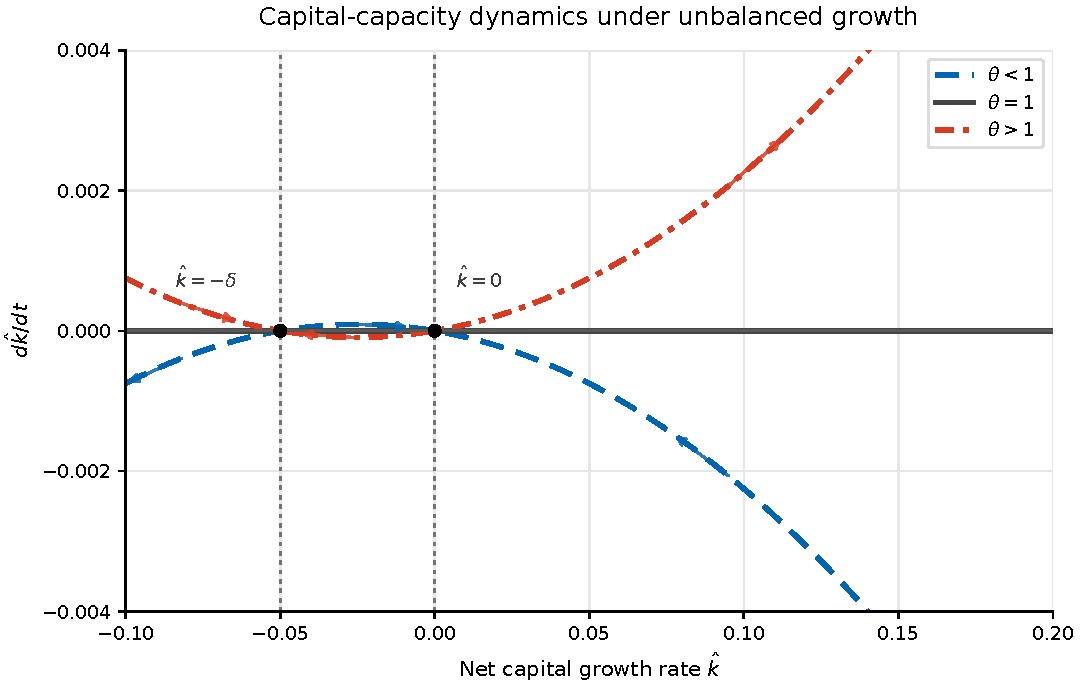
\includegraphics[width=0.92\linewidth]{figures/fig_S3_phase_diagram_capital_capacity_dynamics.pdf}
\caption*{\footnotesize Note: Panel A plots the overaccumulation regime ($\theta = 0.8 < 1.0$) where capital acceleration is negative ($d\hat{k}/dt < 0$ for $\hat{k} > -\delta$), pushing the net accumulation rate toward the stable stagnation equilibrium at $\hat{k}^* = -\delta$. Panel B plots the explosive growth regime ($\theta = 1.2 > 1.0$) where capital acceleration is positive ($d\hat{k}/dt > 0$ for $\hat{k} > -\delta$), causing the accumulation rate to diverge. Both panels show the initial condition $\hat{k}_0 = 3\%$ where $d\hat{k}/dt = \mp 0.128\%$, consistent with the numerical example in \S\ref{subsec:balanced_unbalanced_growth}.}
\label{fig:ode_phase_diagram}
\end{figure}

\paragraph{3.21}
While effective demand and distributive conflict are crucial to the broader macroeconomic picture, we abstract from them in this initial formulation to isolate the supply-side mechanics of accumulation. Institutional and macroeconomic forces certainly influence the speed and direction of capital accumulation, but they do not generate the underlying dynamic itself. The differential equations in Appendix~\ref{app:acc_dynamics} demonstrate how the system behaves under different accumulation regimes. However, the empirical single-equation model we will estimate restricts the transformation elasticity ($\theta$) to a constant value over time. The next step is to test whether this assumption of a time-invariant $\theta$ actually holds in the historical data, thereby revealing the limits of this fixed-parameter approach.

\subsection{Trend Stabilization, Viability Condition, and the Double-Misspecification Bias}
\label{subsec:trend_stabilized_closure}

\paragraph{3.22}
We have previously argued that, econometrically, the inclusion of a time trend might absorb variation arising from distributive conflict and distinct historical configurations. Hence, we analyze the inclusion of a time trend under an unbalanced growth closure ($g_{Y^p} = \theta g_K$) and its consequences for dynamic stability. As established in the phase dynamics, a system experiencing overaccumulation ($\theta < 1$) forces the net accumulation rate to decay to zero. Using the same accounting identities that drive dynamic stability, we can show that introducing a deterministic level trend ($b$) under an unbalanced growth closure ($g_{Y^p} = \theta g_K + b$) stabilizes the system.

\paragraph{3.23}
Substituting this extended closure into the acceleration identity transforms the system into a quadratic ordinary differential equation:
\begin{equation}
\frac{d\hat{k}}{dt} = (\hat{k} + \delta)\left[(\theta - 1)\hat{k} + b\right].
\end{equation}

\paragraph{3.24}
This specification shifts the equilibrium structure of the accumulation process. The stagnation limit ($\hat{k}^* = 0$) is replaced by a new interior root:
\begin{equation}
\hat{k}^* = \frac{b}{1 - \theta}.
\end{equation}

\paragraph{3.25}
Under overaccumulation ($\theta < 1$) with positive autonomous technical progress ($b > 0$), this interior equilibrium is locally stable. The depreciation rate ($\delta$) anchors the negative root, while the ratio $b / (1 - \theta)$ scales autonomous progress against the structural imbalance, preventing stagnation. Conversely, in the excess capacity regime ($\theta > 1$), the deterministic trend $b$ fails to provide a stabilizing anchor. Because $(1 - \theta)$ is negative, the interior root $\hat{k}^* = b / (1 - \theta)$ becomes negative, meaning no economically meaningful positive steady-state accumulation rate exists. Instead of stabilizing the system, the trend $b$ merely compounds the dynamic divergence, exacerbating the explosive trajectory where productive capacity continuously outpaces capital accumulation and reinforcing the chronic excess capacity that ultimately requires exogenous autonomous demand to resolve.

\paragraph{3.26}
The analysis of technical change by \citet{Basu2022} demonstrates why treating the trend-stabilized steady state as a smooth, exogenously determined path is fundamentally problematic. Basu establishes that under capitalism, technical change is not a neutral, exogenous drift but is governed by the strict filter of \textit{capitalist viability}: producers only adopt new techniques if they reduce costs at prevailing prices and real wages. Crucially, the trajectory and specific type of technical change---whether it is capital-using, labor-saving (CU-LS), or capital-saving, labor-saving (CS-LS)---are not predetermined. Instead, they are endogenously shaped by the balance of class struggle over the real wage relative to productivity growth. Therefore, the deterministic trend coefficient ($b$) in the capacity-capital ratio does not represent autonomous technological progress. Rather, it is the econometric residue of the feedback loop between distributional conflict and the choice of technique. In other words, imposing a time trend masks how class struggle actively and endogenously reshapes the ceiling of productive capacities.

\paragraph{3.27}
The statistical validity of the capacity utilization series relies on establishing a stable cointegrating relation between output, capital, and the deterministic trend. Omitting distributive conflict while including the exogenous trend introduces a double misspecification. As \citet{Basu2020} demonstrates, when an econometric model excludes a relevant variable—in this case, distributive conflict and its influence on the choice of technique \citep{Kurz1986}—while including an irrelevant proxy like a deterministic time trend, the estimator for the capital coefficient suffers from compound bias. Because the trend mathematically absorbs the unobserved shifts in distribution, this indirect bias channel compromises the recovered elasticity parameter $\theta$, making it a passive statistical fit rather than a stable production relation.

\paragraph{3.28}
Estimating this relation over Shaikh's sample imposes rigid temporal constraints. This restriction forces both the elasticity ($\theta$) and the trend ($b$) to act as time-invariant constants across shifting institutional configurations. The classical long-run closure ($\mu = 1$) isolates theoretical capital-to-capacity relations \citep{Foley1985} or smooth reproduction paths \citep{Okishio2022, Basu2022}. Because real capitalist economies routinely violate these strict proportionality conditions, imposing time-invariance forces the recovered parameters to mathematically average across structurally heterogeneous historical periods.

\paragraph{3.29}
Looking at the actual post-war historical trajectory of the US corporate sector (1947--2011) using the original data tables by \citet{Shaikh2016}, these theoretical regimes correspond to distinct accumulation phases. During the Post-War Golden Age (1947--1973), the US corporate sector experienced rapid capital accumulation alongside strong output growth, with the real gross capital stock expanding at an average annual rate of 5.4\% and real gross value added growing at 4.4\%. This period represents a relatively balanced accumulation path with a high, stable output--capital ratio. During the transition of the stagflation crisis (1974--1982), the growth of the real capital stock remained relatively high at 4.8\% (driven by energy-related investments and structural restructuring), while real output growth slowed significantly to 2.7\%, causing the output-capital ratio to collapse. Subsequently, in the neoliberal era (1983--2011), the rate of capital accumulation fell to an average of 3.3\% annually, while real output grew at only 2.7\%, leaving the output--capital ratio volatile and structurally depressed. This empirical shift in how capital accumulation translates to productive capacity strongly suggests a change in the underlying transformation elasticity $\theta$ across these eras. Imposing a time-invariant parameter over this entire 64-year span forces the econometric model to mathematically average across these structurally distinct historical periods, actively masking the very crises and regime shifts that define capitalist development.

\paragraph{3.30}
This parametric averaging also bears directly on the classical debate concerning the long-run endogeneity of capital accumulation to aggregate demand. In the Neo-Kaleckian framework, capacity utilization is endogenous to demand in the long run, and investment adjusts to minimize utilization gaps. Conversely, the Sraffian position (e.g., the Supermultiplier model) treats the choice of technique and the capital accumulation path as weakly exogenous to demand-led capacity disequilibrium, adjusting instead to cost-minimizing criteria at a given real wage. Our conceptualization of unbalanced growth ($\theta \neq 1.0$) introduces a more nuanced, counteracting dynamic to this debate. Under overaccumulation ($\theta < 1.0$), capital accumulation is structurally unstable, meaning that the capacity ceiling grows slower than capital stock. While this decoupling implies that investment is weakly exogenous to short-run capacity utilization errors, the system-level instability prevents simple long-run demand adaptation. Crucially, if the weak exogeneity of investment and the secular instability of overaccumulation act as counteracting forces, they may cancel each other out. This counteracting dynamic represents a plausible interpretation that might obscure the resolution of the Sraffian and Neo-Kaleckian debates themselves---an analytical blind spot explained by both frameworks operating under the restrictive assumption of a balanced-growth path with a fixed output--capital ratio.

\paragraph{3.31}
The next section~\ref{sec:replication_strategy} implements an analytical stress test across three distinct stages to identify the conditions under which Shaikh's single-equation ARDL estimation fails to identify cointegration. Stage S0 establishes a baseline of reproducibility using the original data tables by \citet{Shaikh2016} and lag lengths. Stage S1 implements an admissibility test by estimating a grid of 500 ARDL specifications, mapping parameter sensitivity to researcher choices—such as lag structures, information-criterion penalties, and historical dummy variables. Stage S2 estimates the long-run relationship using a Vector Error Correction Model (VECM) to determine whether joint system stability holds in a bivariate setting, or if it requires the logged rate of exploitation ($e_t = \ln[\pi_t / (1 - \pi_t)]$ ) to establish a stable cointegrating relationship.
